\chapter{Introduction}
Research on congestion control has not only remained vibrant since the 1980s, but has flourished in recent years as new applications, network technologies, and workload patterns have been emerging at a rapid rate. Figure~\ref{fig:cctimeline} shows a time-line of innovations in this area.

At its core, a congestion control protocol determines when each segment of data must be sent. Because a natural place to make this decision is within the transport layer, congestion control today is tightly woven into kernel TCP software and runs independently for each TCP connection.

This design has three shortcomings. First, many modern proposals use techniques such as Bayesian forecasts (Sprout~\cite{sprout}), offline or online learning (Remy~\cite{remy}, PCC~\cite{pcc}, PCC-Vivace~\cite{pcc-vivace}, Indigo~\cite{pantheon}), or signal processing with Fourier transforms (Nimbus~\cite{nimbus}) that are difficult, if not impossible, to implement in a kernel lacking useful libraries for the required calculations. For example, computing the cube root function in Linux's Cubic implementation requires using a table lookup and a Newton-Raphson iteration instead of a simple function call. Moreover, to meet tight performance constraints, in-kernel congestion control methods have largely been restricted to simple window or rate arithmetic.

%However, this tight coupling is not fundamental to congestion control; rather,
%it imposes an artificial restriction on algorithms to restrict their
%computations to a single packet inter-arrival time lest they slow down the
%flow.
%Research on congestion control is flourishing, and newly proposed algorithms lacking kernel %implementations, such as
%PCC-Vivace~\cite{pcc-vivace}, Nimbus~\cite{nimbus}, Remy~\cite{remy}, and
%Sprout~\cite{sprout}, 
%all involve calculations that are cumbersome to perform in
%he kernel and challenging to engineer to meet tight performance
%requirements.
%For example, Nimbus uses Fast Fourier Transforms to determine the amount and
%nature of the cross-traffic on the bottleneck link.

Second, the kernel TCP stack is but one example of a {\em datapath}, the term we use for any module that provides data transmission and reception interfaces between higher-layer applications and lower-layer network hardware. Recently, new datapaths have emerged, including user-space protocols atop UDP (e.g., QUIC~\cite{quic}, WebRTC~\cite{webrtc}, Mosh~\cite{mosh}), kernel-bypass methods (e.g., mTCP/DPDK~\cite{dpdk,mtcp,netmap}), RDMA~\cite{dcqcn}, multi-path TCP (MPTCP)~\cite{mptcp}, and specialized Network Interface Cards (``SmartNICs''~\cite{smartnic}). This trend suggests that future applications will use datapaths different from traditional kernel-supported TCP connections.

\begin{figure}[t]
\centering
    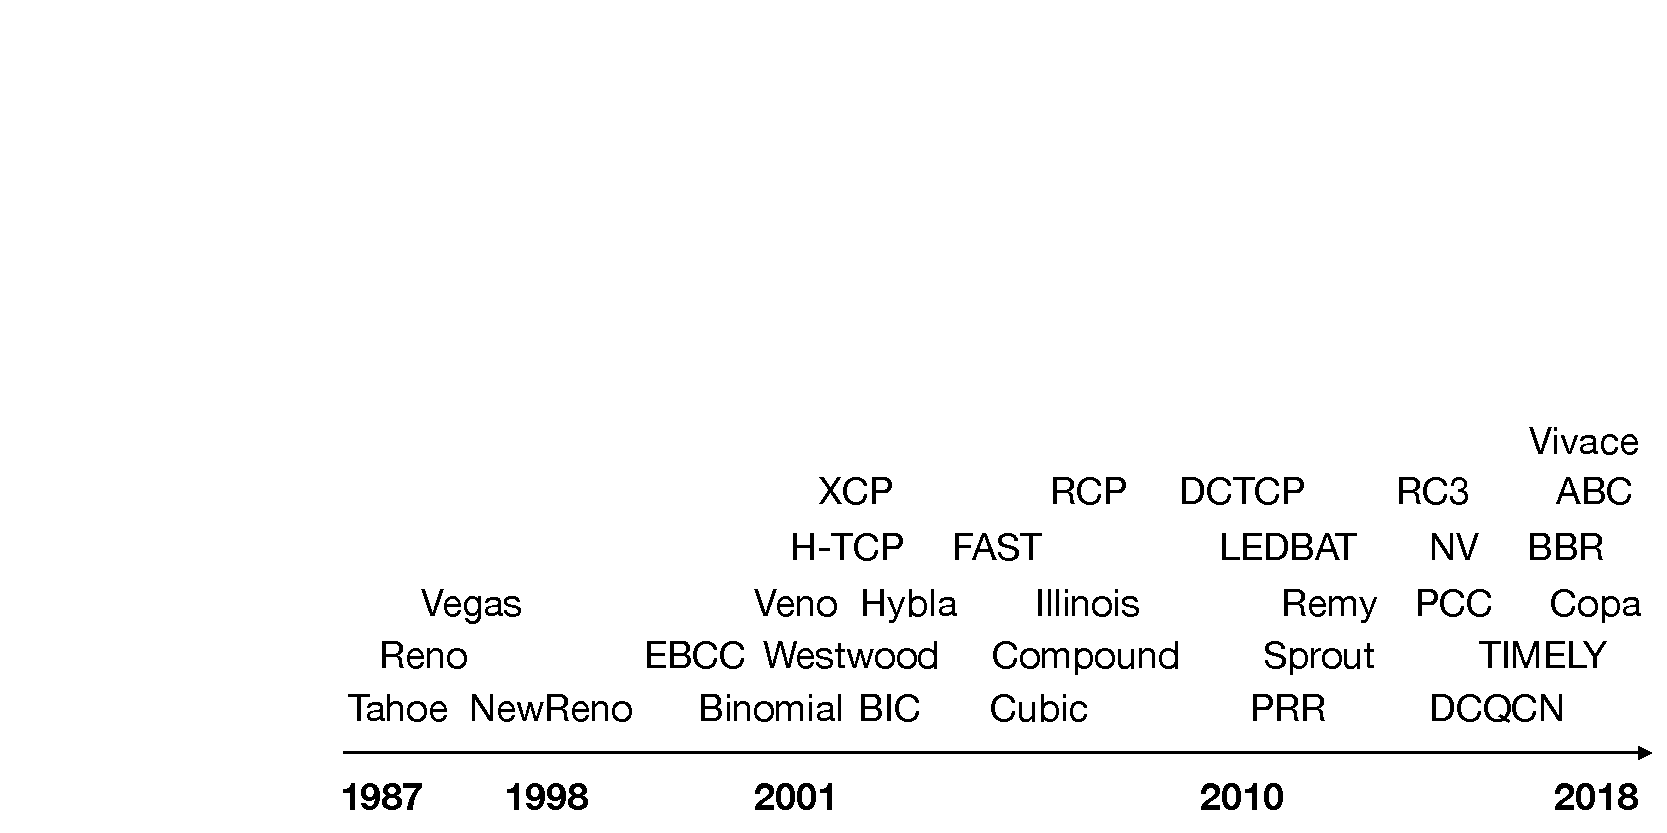
\includegraphics[width=\columnwidth]{img/cc-timeline-nocongsig}
    %\vspace{-20pt}
    %\caption{Congestion control algorithms over the years.}
    \caption{As link characteristics diversify, developers have developed a battery of congestion control algorithms, from the ``long-fat pipe'' schemes of the mid-2000s~\cite{westwood, veno, htcp, hybla} to purely delay-based~\cite{vegas, fasttcp, ledbat, nv, timely} and hybrid loss-delay~\cite{illinois, compound} schemes, and more recent proposals~\cite{pcc, remy, sprout, bbr, copa, abc}.}\label{fig:cctimeline}
    %\vspace{-16pt}
\end{figure}

New datapaths offer limited choices for congestion control because implementing these algorithms correctly takes considerable time and effort. 
We believe this significantly hinders experimentation and innovation both in the datapaths and the congestion control algorithms running over them.
For instance, the set of currently available algorithms in mTCP~\cite{mtcp}, a TCP implementation on DPDK, is limited to a variant of Reno. 
QUIC, despite Google's imposing engineering resources, does not have implementations of several algorithms that have existed in the Linux kernel for many years.  
We expect this situation to worsen with the emergence of new hardware accelerators and programmable network interface cards (NICs) because high-speed hardware designers tend to forego programming convenience for performance. 
%The difficulty is not the volume of code, but rather is the subtle correctness and performance issues in various algorithms that require expertise to understand and resolve.

Third, tying congestion control tightly to the datapath makes it hard to provide new capabilities, such as aggregating congestion information across flows that share common bottlenecks, as proposed in the Congestion Manager project~\cite{cm}. 

%This paper starts from the observation that congestion control algorithms need not be implemented in the datapath. 

\smallskip
If, instead, the datapath encapsulated the information available to it about {\em congestion signals} like packet round-trip times (RTT), receptions, losses, ECN, etc., and periodically provided this information to an off-datapath module, then congestion control algorithms could run in the context of that module. 
By exposing an analogous interface to control transmission parameters such as the window size, pacing rate, and transmission pattern, the datapath could transmit data according to the policies specified by the off-datapath congestion control algorithm. Of course, the datapath must be modified to expose
such an interface, but this effort needs to be undertaken only once for each datapath.
%, and does not grow with the number of congestion control algorithms.

We use the term {\em Congestion Control Plane (CCP)} to refer to this off-datapath module. Running congestion control in the CCP offers the following benefits:
\begin{enumerate}
    \item {\bf Write-once, run-anywhere:} One can write a congestion control algorithm once and run it on any datapath that supports the specified interface. 
    We describe several algorithms running on three datapaths: the Linux kernel, mTCP/DPDK, and QUIC, and show algorithms running for the first time on certain datapaths (e.g., Cubic on mTCP/DPDK and Copa on QUIC).
    \item {\bf Higher pace of development:} With good abstractions,
      a congestion control designer can focus on the algorithmic essentials
      without worrying about the details and data structures of the
      datapath. The resulting code is easier to read and maintain. In our implementation, congestion control algorithms in CCP are written in Rust or Python and run in user space. 
    \item {\bf New capabilities:} CCP makes it easier to provide new
      capabilities, such as aggregate control of multiple flows~\cite{cm}, and algorithms that require sophisticated computation (e.g., signal processing, machine learning, \etc) running in \userspace programming environments. 
      %These algorithms are hard to write as window updates on incoming ACKs.
      %All the benefits of a \userspace programming environment (libraries, debuggers, \etc) will be available to       developers.
\end{enumerate}

%\vspace{0.1in}
\smallskip 
This paper's contributions include:

\begin{itemize}
\item An event-driven language to specify congestion control
  algorithms. Algorithm developers specify congestion control behavior using
  combinations of events and conditions, such as the receipt of an
  ACK or a loss event, along with corresponding handlers to perform
  simple computations directly in the datapath (\eg increment the window) or defer
  complex logic to a \userspace component. We show how to implement several recently proposed algorithms and also congestion-manager aggregation. 

\item A specification of datapath responsibilities. These include congestion
  signals that a datapath should maintain (Table~\ref{tab:api}), as
  well as a simple framework to execute directives from a CCP program. This
  design enables ``write-once, run-anywhere'' protocols.

%\item A demonstration of new capabilities enabled by CCP, including
%   new congestion control algorithms and the implementation of an
%  aggregate congestion controller acting on behalf of multiple flows.

\item An evaluation of the fidelity of CCP relative to in-kernel
  implementations under a variety of link conditions. Our CCP implementation
  matches the performance of Linux kernel implementations at only a small
  overhead (5\% higher CPU utilization in the worst case).
%  Furthermore, we show it  is feasible to implement infrequent congestion control even in low-RTT, high
  % bandwidth environments.

\end{itemize}
